\documentclass{beamer}

\usepackage{graphicx,hyperref,udesc,url}
\usepackage{amsmath,amsthm,amsfonts,amssymb}
\usepackage{latexsym}
\usepackage{graphicx,udesc,url}
\usepackage[utf8]{inputenc}
\usepackage[T1]{fontenc}
\usepackage{booktabs}
\usepackage{gensymb}
\usepackage{amsmath,amssymb,proof}
\usepackage{booktabs}
\usepackage{dirtree}
\usepackage{listings}
\usepackage{lmodern}

\definecolor{green-hl}{RGB}{54,88,65}
\newcommand{\hl}[1]{{\color{white}\colorbox{green-hl}{#1}}}

\definecolor{mygrey}{gray}{0.85}

\newcommand{\prog}[1]{
  \normalfont\ttfamily
  \begin{center}\begin{tabular}{l}
       #1
  \end{tabular} \end{center}
  \normalfont}

\newcommand{\proga}[1]{
 \normalfont\ttfamily
  \begin{tabbing}
        #1
   \end{tabbing}
 \normalfont}

\newcommand{\progfig}[1]{\parbox{.96\textwidth}{
  \normalfont\ttfamily
  {\small
  \parbox{\textwidth}{\begin{tabbing}
        #1
  \end{tabbing}}
}
  \normalfont}}

\newcommand{\progfigmed}[1]{\parbox{.65\textwidth}{
  \normalfont\ttfamily
  {\small
  \parbox{\textwidth}{\begin{tabbing}
        #1
  \end{tabbing}}
}
  \normalfont}}


\newcommand{\progfigsmall}[1]{\parbox{.44\textwidth}{
  \normalfont\ttfamily
  {\small
%  \begin{center}
  \parbox{.44\textwidth}{\begin{tabbing}
        #1
  \end{tabbing}}
%  \end{center}
}
  \normalfont}}

\newcommand{\progb}[1]{
  \normalfont\ttfamily
  {\small
  \begin{center}
  \parbox{\textwidth}{\begin{tabbing}
        #1
  \end{tabbing}}
  \end{center} }
  \normalfont}

\newcommand{\scripttag}[1]{\texttt{\scriptsize{(}}\textsl{\scriptsize{#1}}{\texttt{\scriptsize{)}}}}

\newcommand{\progn}[1]{
  \begin{center}
  \parbox{\textwidth}{\begin{tabbing}
        #1
  \end{tabbing}}
  \end{center} }



\newcommand{\progbb}[1]{
  \normalfont\ttfamily
  \begin{center}
  \shadowbox{\parbox{\textwidth}{\begin{tabbing}
        #1
  \end{tabbing}}}
  \end{center}
  \normalfont}

\newcommand{\progc}[1]{
  \normalfont\ttfamily
  \begin{center}
  \fbox{\parbox{\textwidth}{\begin{tabbing}
        #1
  \end{tabbing}}}
  \end{center}
  \normalfont}

\newcommand{\progcc}[1]{
  \normalfont\ttfamily
  \begin{center}
  \fbox{\begin{tabular}{p{4cm}}
        #1
  \end{tabular}}
  \end{center}
  \normalfont}

\newcommand{\progaa}[1]{
  \normalfont\ttfamily
  \begin{center}\begin{tabular}{ll}
       #1
  \end{tabular} \end{center}
  \normalfont}

\newcommand{\progaaa}[1]{
  \normalfont\ttfamily
  \begin{center}\begin{tabular}{lll}
       #1
  \end{tabular} \end{center}
  \normalfont}

\newcommand{\progeq}[1]{
  \normalfont\ttfamily
  \begin{center}\begin{tabular}{rcl}
       #1
  \end{tabular} \end{center}
  \normalfont}

\newcommand{\CT}{\text{\it CT\/}}
\newcommand{\CSSAT}{\text{\it CS-SAT\/}}
\newcommand{\ssat}{\text{\tt sat}}

\newcommand{\lcg}{\text{\it lcg\/}}

\newcommand{\Integer}{\text{\it Integer\/}}
\newcommand{\Bool}{\text{\it Bool\/}}
\newcommand{\Int}{\text{\it Int\/}}
\newcommand{\Char}{\text{\it Char\/}}
\newcommand{\Float}{\text{\it Float\/}}
\newcommand{\Double}{\text{\it Double\/}}

\newcommand{\True}{\text{\it True\/}}
\newcommand{\False}{\text{\it False\/}}

\newcommand{\Lit}{\text{\it Lit\/}}
\newcommand{\Inc}{\text{\it Inc\/}}
\newcommand{\IsZ}{\text{\it IsZ\/}}
\newcommand{\If}{\text{\it If\/}}
\newcommand{\Pair}{\text{\it Pair\/}}
\newcommand{\Term}{\text{\it Term\/}}

\newcommand{\eval}{\text{\it eval\/}}
\newcommand{\iinsert}{\text{\it insert\/}}

\newcommand{\MMo}{{\tt MMo}}

\newcommand{\genn}[1]{\bar{\bar{#1}}}
\newcommand{\abrgenn}[1]{\|#1\|}

\newcommand{\T}{\text{\it T\/}}
\newcommand{\Tu}{\text{\it T1\/}}
\newcommand{\Td}{\text{\it T2\/}}
\newcommand{\test}{\text{\it test\/}}
\newcommand{\sat}{\text{\it sat\/}}
\newcommand{\sats}{\text{\it sats\/}}

\newcommand{\Eq}{\text{\it Eq\/}}

\newcommand{\TEq}{\rightarrowtail}}
\newcommand{\TEqD}{\rotatebox[origin=c]{270}{\Large \rightarrowtail}}
\newcommand{\tti}{\texttt{i}}
\newcommand{\ttk}{\texttt{k}}
\newcommand{\ttx}{\texttt{x}}
\newcommand{\tty}{\texttt{y}}
\newcommand{\ttp}{\texttt{p}}
\newcommand{\tts}{\texttt{s}}
\newcommand{\ttr}{\texttt{r}}
\newcommand{\tta}{\texttt{a}}
\newcommand{\ttc}{\texttt{c}}
\newcommand{\ttconst}{\texttt{const}}
\newcommand{\ttinfo}{\texttt{info}}

% \newcommand{\INST}{\text{\tt INST}}
% \newcommand{\ABS}{\text{\tt ABS}}
% \newcommand{\GEN}{\text{\tt GEN}}
% \newcommand{\VAR}{\text{\tt VAR}}
% \newcommand{\PVAR}{\text{\tt PVAR}}
% \newcommand{\SKO}{\text{\tt VAR-SKO}}
% \newcommand{\UNI}{\text{\tt VAR-UNI}}
% \newcommand{\FUN}{\text{\tt FUN}}
% \newcommand{\CONS}{\text{\tt CONS}}
% \newcommand{\LAM}{\text{\tt LAM}}
% \newcommand{\APP}{\text{\tt APP}}
% \newcommand{\LET}{\text{\tt LET}}
% \newcommand{\LETA}{\text{\tt LETA}}
% \newcommand{\CASE}{\text{\tt CASE}}
% \newcommand{\BIND}{\text{\tt BIND}}
% \newcommand{\EEMPTY}{\text{\tt EMPTY}}
% \newcommand{\IMPROVE}{\text{\tt IMPROVE}}
% \newcommand{\PATVAR}{\text{\tt PAT-VAR}}
% \newcommand{\PAT}{\text{\tt PAT}}
% \newcommand{\TPAT}{\text{\tt TPAT}}
% \newcommand{\INFER}{\text{\tt INFER}}
% \newcommand{\PATCONS}{\text{\tt PAT-CONS}}
% \newcommand{\ALTS}{\text{\tt ALTS}}
% \newcommand{\ALT}{\text{\tt ALT}}
% \newcommand{\MAIN}{\text{\tt MAIN}}
% \newcommand{\alts}{\text{\tt alts}}
% \newcommand{\alt}{\text{\tt alt}}
% \newcommand{\pat}{\text{\tt pat}}

%%%%%%%%%%%%%%%%%%%%%%%%%%%%%%%%%%%%%%%%%%%%%%%%%%%%%%%%%%%%%%%%%%%%%%%%%%%%%
%                                                                           %
% DEFINITIONS OF SYMBOL-PRODUCING COMMANDS                                  %
%                                                                           %
%    TLA+      LaTeX                                                        %
%    symbol    command                                                      %
%    ------    -------                                                      %
%    =>        \implies                                                     %
%    <:        \ltcolon                                                     %
%    :>        \colongt                                                     %
%    ==        \defeq                                                       %
%    ..        \dotdot                                                      %
%    ::        \coloncolon                                                  %
%    =|        \eqdash                                                      %
%    ++        \pp                                                          %
%    --        \mm                                                          %
%    **        \stst                                                        %
%    //        \slsl                                                        %
%    ^         \ct                                                          %
%    \A        \A                                                           %
%    \E        \E                                                           %
%    \AA       \AA                                                          %
%    \EE       \EE                                                          %
%%%%%%%%%%%%%%%%%%%%%%%%%%%%%%%%%%%%%%%%%%%%%%%%%%%%%%%%%%%%%%%%%%%%%%%%%%%%%
% \newcommand{\implies}{\Rightarrow}
\newcommand{\ltcolon}{\mathrel{<\!\!\mbox{:}}}
\newcommand{\colongt}{\mathrel{\!\mbox{:}\!\!>}}
\newcommand{\defeq}{\;\mathrel{\smash   %% keep this symbol from being too tall
    {{\stackrel{\scriptscriptstyle\Delta}{=}}}}\;}
\newcommand{\dotdot}{\mathrel{\ldotp\ldotp}}
\newcommand{\coloncolon}{\mathrel{::\;}}
\newcommand{\eqdash}{\mathrel = \joinrel \hspace{-.28em}|}
\newcommand{\pp}{\mathbin{++}}
\newcommand{\mm}{\mathbin{--}}
\newcommand{\stst}{*\!*}
\newcommand{\slsl}{/\!/}
\newcommand{\ct}{\hat{\hspace{.4em}}}
\newcommand{\A}{\forall}
\newcommand{\E}{\exists}
\renewcommand{\AA}{\makebox{$\raisebox{.05em}{\makebox[0pt][l]{%
   $\forall\hspace{-.517em}\forall\hspace{-.517em}\forall$}}%
   \forall\hspace{-.517em}\forall \hspace{-.517em}\forall\,$}}
\newcommand{\EE}{\makebox{$\raisebox{.05em}{\makebox[0pt][l]{%
   $\exists\hspace{-.517em}\exists\hspace{-.517em}\exists$}}%
   \exists\hspace{-.517em}\exists\hspace{-.517em}\exists\,$}}
\newcommand{\whileop}{\.{\stackrel
  {\mbox{\raisebox{-.3em}[0pt][0pt]{$\scriptscriptstyle+\;\,$}}}%
  {-\hspace{-.16em}\triangleright}}}

% Commands are defined to produce the upper-case keywords.
% Note that some have space after them.
\newcommand{\TLA}{TLA\textsuperscript{+} }
\newcommand{\TLAA}{TLA\textsuperscript{+}}
\newcommand{\FANCYA}{\textbf{$\mathcal{A}$} }
\newcommand{\FANCYAA}{\textbf{$\mathcal{A}$}}
\newcommand{\trabalhando}{"trabalhando"}
\newcommand{\preparado}{"preparado"}
\newcommand{\cometido}{"cometido"}
\newcommand{\abortado}{"abortado"}

\newcommand{\ASSUME}{\textsc{assume }}
\newcommand{\ASSUMPTION}{\textsc{assumption }}
\newcommand{\AXIOM}{\textsc{axiom }}
\newcommand{\BOOLEAN}{\textsc{boolean }}
\newcommand{\CASE}{\textsc{case }}
\newcommand{\CONSTANT}{\textsc{constant }}
\newcommand{\CONSTANTS}{\textsc{constants }}
\newcommand{\ELSE}{\settowidth{\symlength}{\THEN}%
   \makebox[\symlength][l]{\textsc{ else}}}
\newcommand{\EXCEPT}{\textsc{ except }}
\newcommand{\EXTENDS}{\textsc{extends }}
\newcommand{\FALSE}{\textsc{false}}
\newcommand{\IF}{\textsc{if }}
\newcommand{\IN}{\settowidth{\symlength}{\LET}%
   \makebox[\symlength][l]{\textsc{in}}}
\newcommand{\INSTANCE}{\textsc{instance }}
\newcommand{\LET}{\textsc{let }}
\newcommand{\LOCAL}{\textsc{local }}
\newcommand{\MODULE}{\textsc{module }}
\newcommand{\OTHER}{\textsc{other }}
\newcommand{\STRING}{\textsc{string}}
\newcommand{\THEN}{\textsc{ then }}
\newcommand{\THEOREM}{\textsc{theorem }}
\newcommand{\LEMMA}{\textsc{lemma }}
\newcommand{\PROPOSITION}{\textsc{proposition }}
\newcommand{\COROLLARY}{\textsc{corollary }}
\newcommand{\TRUE}{\textsc{true}}
\newcommand{\VARIABLE}{\textsc{variable}}
\newcommand{\VARIABLES}{\textsc{variables}}
\newcommand{\WITH}{\textsc{ with }}
\newcommand{\WF}{\textrm{WF}}
\newcommand{\SF}{\textrm{SF}}
\newcommand{\CHOOSE}{\textsc{choose }}
\newcommand{\ENABLED}{\textsc{enabled }}
\newcommand{\UNCHANGED}{\textsc{unchanged }}
\newcommand{\SUBSET}{\textsc{subset }}
\newcommand{\UNION}{\textsc{union }}
\newcommand{\DOMAIN}{\textsc{domain }}
% Added for tla2tex
\newcommand{\BY}{\textsc{by }}
\newcommand{\OBVIOUS}{\textsc{obvious }}
\newcommand{\HAVE}{\textsc{have }}
\newcommand{\QED}{\textsc{qed }}
\newcommand{\TAKE}{\textsc{take }}
\newcommand{\DEF}{\textsc{ def }}
\newcommand{\HIDE}{\textsc{hide }}
\newcommand{\RECURSIVE}{\textsc{recursive }}
\newcommand{\USE}{\textsc{use }}
\newcommand{\DEFINE}{\textsc{define }}
\newcommand{\PROOF}{\textsc{proof }}
\newcommand{\WITNESS}{\textsc{witness }}
\newcommand{\PICK}{\textsc{pick }}
\newcommand{\DEFS}{\textsc{defs }}
\newcommand{\PROVE}{\settowidth{\symlength}{\ASSUME}%
   \makebox[\symlength][l]{\textsc{prove}}\@s{-4.1}}%
  %% The \@s{-4.1) is a kludge added on 24 Oct 2009 [happy birthday, Ellen]
  %% so the correct alignment occurs if the user types
  %%   ASSUME X
  %%   PROVE  Y
  %% because it cancels the extra 4.1 pts added because of the
  %% extra space after the PROVE.  This seems to works OK.
  %% However, the 4.1 equals Parameters.LaTeXLeftSpace(1) and
  %% should be changed if that method ever changes.
\newcommand{\SUFFICES}{\textsc{suffices }}
\newcommand{\NEW}{\textsc{new }}
\newcommand{\LAMBDA}{\textsc{lambda }}
\newcommand{\STATE}{\textsc{state }}
\newcommand{\ACTION}{\textsc{action }}
\newcommand{\TEMPORAL}{\textsc{temporal }}
\newcommand{\ONLY}{\textsc{only }}              %% added by LL on 2 Oct 2009
\newcommand{\OMITTED}{\textsc{omitted }}        %% added by LL on 31 Oct 2009
% \newcommand{\@pfstepnum}[2]{\ensuremath{\langle#1\rangle}\textrm{#2}}
\newcommand{\bang}{\@s{1}\mbox{\small !}\@s{1}}


% \lstset{
%     numbers=left,                   % where to put the line-numbers
%     numberstyle=\small \ttfamily \color[rgb]{0.4,0.4,0.4},
%                 % style used for the linenumbers
%     showspaces=false,               % show spaces adding special underscores
%     showstringspaces=false,         % underline spaces within strings
%     showtabs=false,                 % show tabs within strings adding particular underscores
%     frame=lines,                    % add a frame around the code
%     tabsize=4,                        % default tabsize: 4 spaces
%     breaklines=false,                % automatic line breaking
%     breakatwhitespace=false,        % automatic breaks should only happen at whitespace
%     basicstyle=\ttfamily,
%     %identifierstyle=\color[rgb]{0.3,0.133,0.133},   % colors in variables and function names, if desired.
%     keywordstyle=\color[rgb]{0.133,0.133,0.6},
%     commentstyle=\color[rgb]{0.133,0.545,0.133},
%     stringstyle=\color[rgb]{0.627,0.126,0.941},
% }

\sloppy

\title[De \TLA para linguagem de programação]{Tradução automática de especificação formal modelada em \TLA para linguagem de programação}

\author[Gabriela M. Mafra]{
    Gabriela Moreira Mafra\\\smallskip
    {\scriptsize Universidade do Estado de Santa Catarina \\\smallskip
    \vspace{-2mm}
    \url{gabrielamoreiramafra@gmail.com}}
}

\begin{document}
  \date{22 de Novembro de 2019}
  \begin{frame}
      \titlepage
  \end{frame}

\tableofcontents

\section{Fundamentos}

\begin{frame}
  \frametitle{Especificação Formal}

  \textbf{Especificar Software é como fazer a planta de um edifício}
  \begin{itemize}
    \item Permite verificações
    \item Serve como base para consulta
    \item Mais fácil de modificar do que o produto final
    \item Vem antes da produção
  \end{itemize}

\end{frame}

\begin{frame}
  \frametitle{Sistemas Concorrentes}

  Um sistema é concorrente quando há mais de uma computação concorrendo pelo mesmo recurso.\medskip

  O resultado pode depender da ordem em que essas computações conseguem os recursos.
  \begin{itemize}
    \item Muitas ordens possíveis
    \item Muitos comportamentos possíveis
  \end{itemize}

  \medskip\textbf{Especificar pode ser ainda mais relevante.}

\end{frame}

\begin{frame}
  \frametitle{Geração de código}

  A implementação - ou a tradução da especificação em linguagem de programação - pode ser feita por um programador ou um tradutor automático.\medskip

  Problemas da tradução manual:
  \begin{itemize}
    \item Suscetível a erro - causando a perda de propriedades verificadas.
    \item Custosa
  \end{itemize}\medskip

  Z, B-Method e ASM (\textit{Abstract State Machine}) tem geradores de código.\medskip

\end{frame}

\begin{frame}
  \frametitle{Temporal Logic of Actions\textsuperscript{+}}

  Linguagem de especificação baseada na lógica TLA.
  \begin{itemize}
    \item Sintaxe matemática
    \item Ideal para especificar sistemas concorrentes
  \end{itemize}\medskip

  Não é disponibilizado um gerador de código.\medskip\pause

  \begin{block}{Objetivo}
    Elaborar um método para gerar código a partir de especificações em \TLA
    \begin{itemize}
      \item Encontrar mapeamentos
      \item Implementar um tradutor, aplicando os mapeamentos e gerando código Elixir
    \end{itemize}
  \end{block}
\end{frame}

\section{\TLA}

\begin{frame}
  \frametitle{TLA}

  TLA = Lógica. \TLA = linguagem de especificação.\medskip

  \begin{block}{Ação}
    Fórmula sobre um passo. Passo = dupla de estados.\\\medskip
    Permite definir quais transições são permitidas.
  \end{block}

  \begin{block}{Comportamento}
    Sequência de passos. Representa uma execução no sistema.\\\medskip
    Uma fórmula é verdadeira para um comportamento se ela é verdadeira para cada passo dele.
  \end{block}

\end{frame}

\section{Gerador de código}

\begin{frame}
  \frametitle{Tradução}
  O método de tradução é descrito através de \textbf{mapeamentos}. Os primeiros mapeamentos definidos foram:
  \begin{itemize}
    \item Ações $\mapsto$ Funções
    \item Estado $\mapsto$ Hash mapeando as variáveis aos seus valores
    \item Ação $\lor$ Ação $\mapsto$ \textbf{Disparo de novo processo}
  \end{itemize}

  \begin{center}
    \Large{Ação $\lor$ Ação}
  \end{center}
    
\end{frame}

\begin{frame}
  \frametitle{Proposta inicial para tradução da disjunção}
  \hspace{-7mm}
  $\progfig{
  ~def main(variaveis) do\\
  ~~~spawn\_link JarrosDeAgua, :main, [grande\_para\_pequeno(variaveis)]\\
  ~~~spawn\_link JarrosDeAgua, :main, [pequeno\_para\_grande(variaveis)]\\
  ~~~spawn\_link JarrosDeAgua, :main, [esvazia\_grande(variaveis)]\\
  ~~~spawn\_link JarrosDeAgua, :main, [esvazia\_pequeno(variaveis)]\\
  ~~~spawn\_link JarrosDeAgua, :main, [enche\_grande(variaveis)]\\
  ~~~spawn\_link JarrosDeAgua, :main, [enche\_pequeno(variaveis)]\\
  ~~~spawn\_link JarrosDeAgua, :main, [variaveis]\\
  ~end\\\\
  ~JarrosDeAgua.main(\%\{\ grande: 0, pequeno: 0 \})
  }$
\end{frame}

\begin{frame}
  \frametitle{Condições e Ações}
  $Sacar(qtd) \defeq \land\ saldo\ \geq qtd$\\
  ~~~~~~~~~~~~~~~~~~~~$\land\ saldo' = saldo - qtd$\\\bigskip
  
  \textbf{Condição de ativação}: $saldo\ \geq qtd$\\
  \textbf{Ação}: $saldo' = saldo - qtd$\\\bigskip\pause
  
  $Next \defeq \lor\ Sacar(10)$\\
  ~~~~~~~~~~~~$\lor\ Sacar(50)$\\\bigskip
  
  Se $saldo = 30$, é possível decidir a próxima ação.\\
  Mas se $saldo = 60$, é necessária uma escolha (não determinismo)\\
\end{frame}

\begin{frame}
  \frametitle{Condições e Ações: Tradução}
  $\progfig{
  ~~def sacar\_condition(variaveis, qtd) do\\
  ~~~~variaveis[:saldo] >= qtd\\
  ~~end\\\\
  ~~def sacar(variaveis, qtd) do\\
  ~~~~\%\{\\
  ~~~~~~saldo: variaveis[:saldo] - qtd,\\
  ~~~~\}\\
  ~~end
  }$
\end{frame}

\begin{frame}
  \frametitle{Banco com problemas de concorrência}
  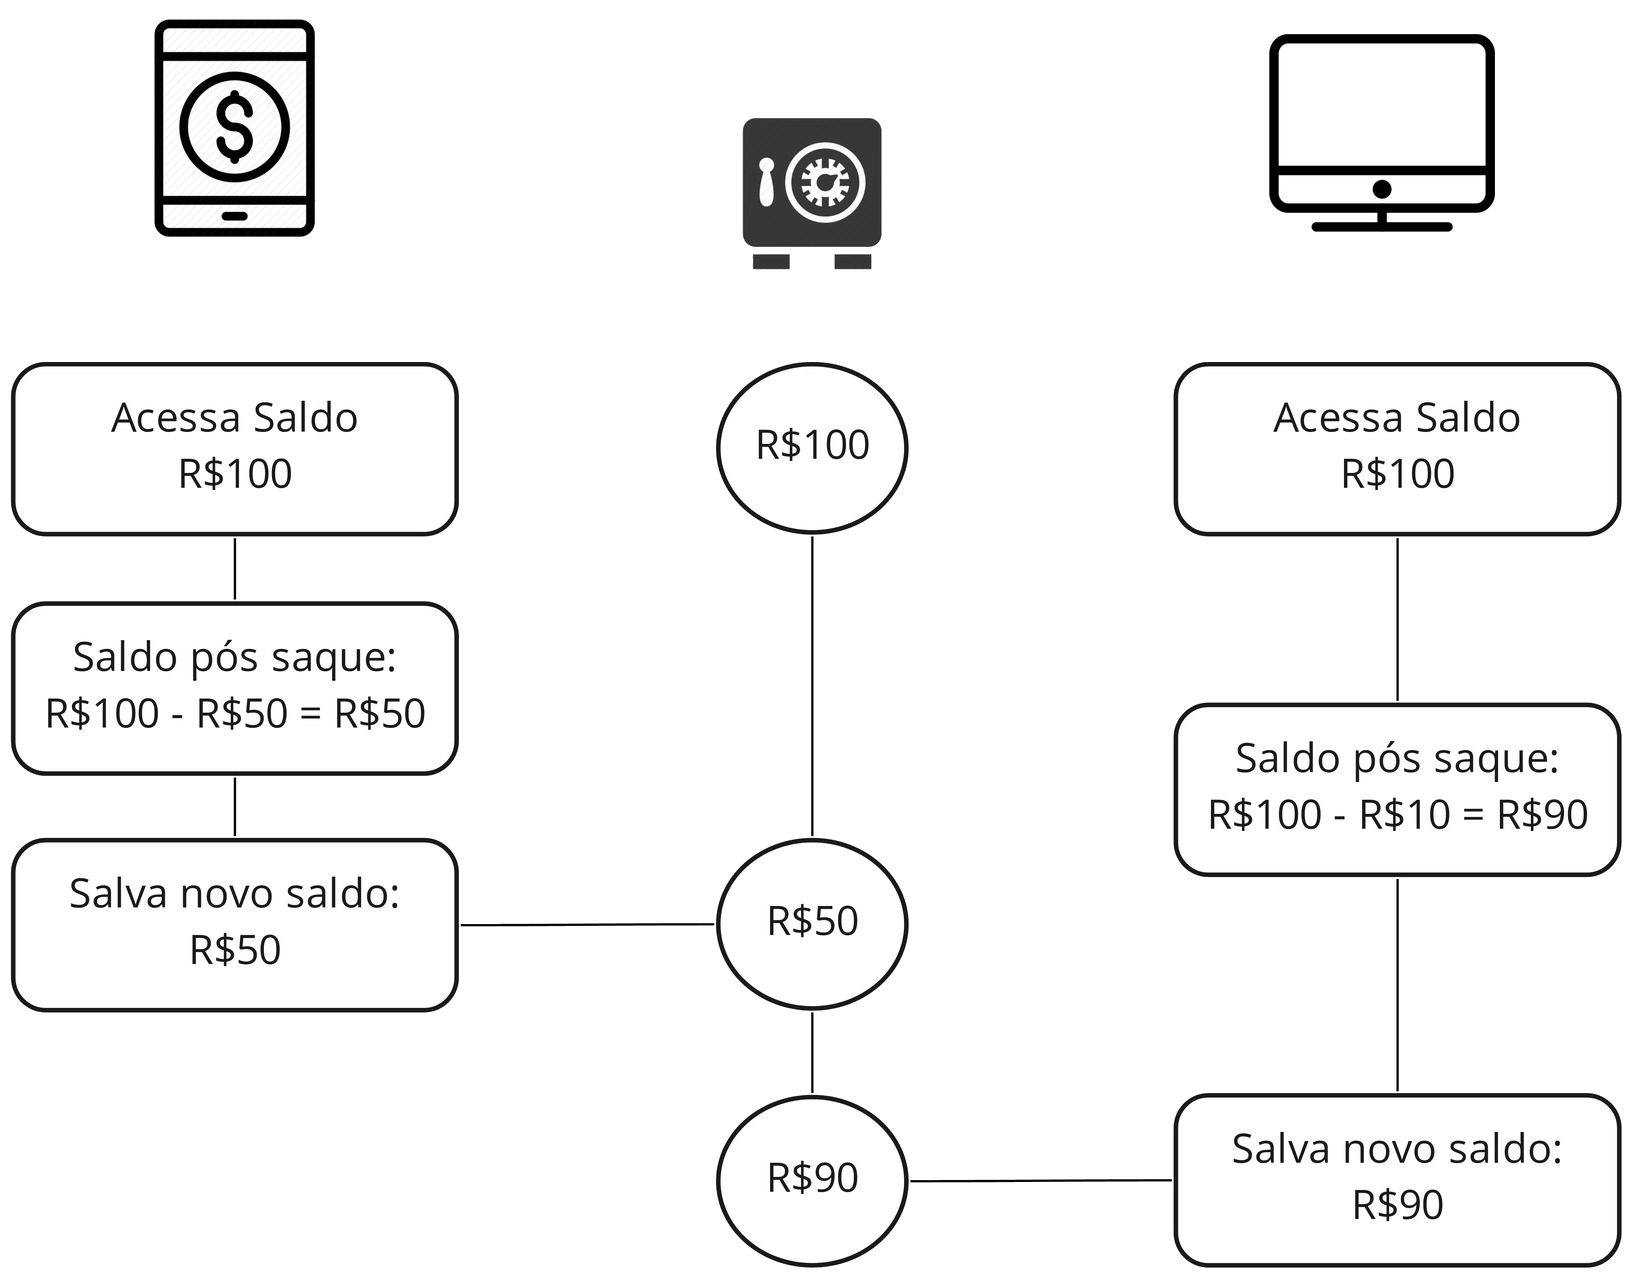
\includegraphics[scale=0.15]{img/bank1.png}
\end{frame}  

\begin{frame}
  \frametitle{Banco modelado em \TLA}

  \begin{minipage}{0.6\textwidth}
  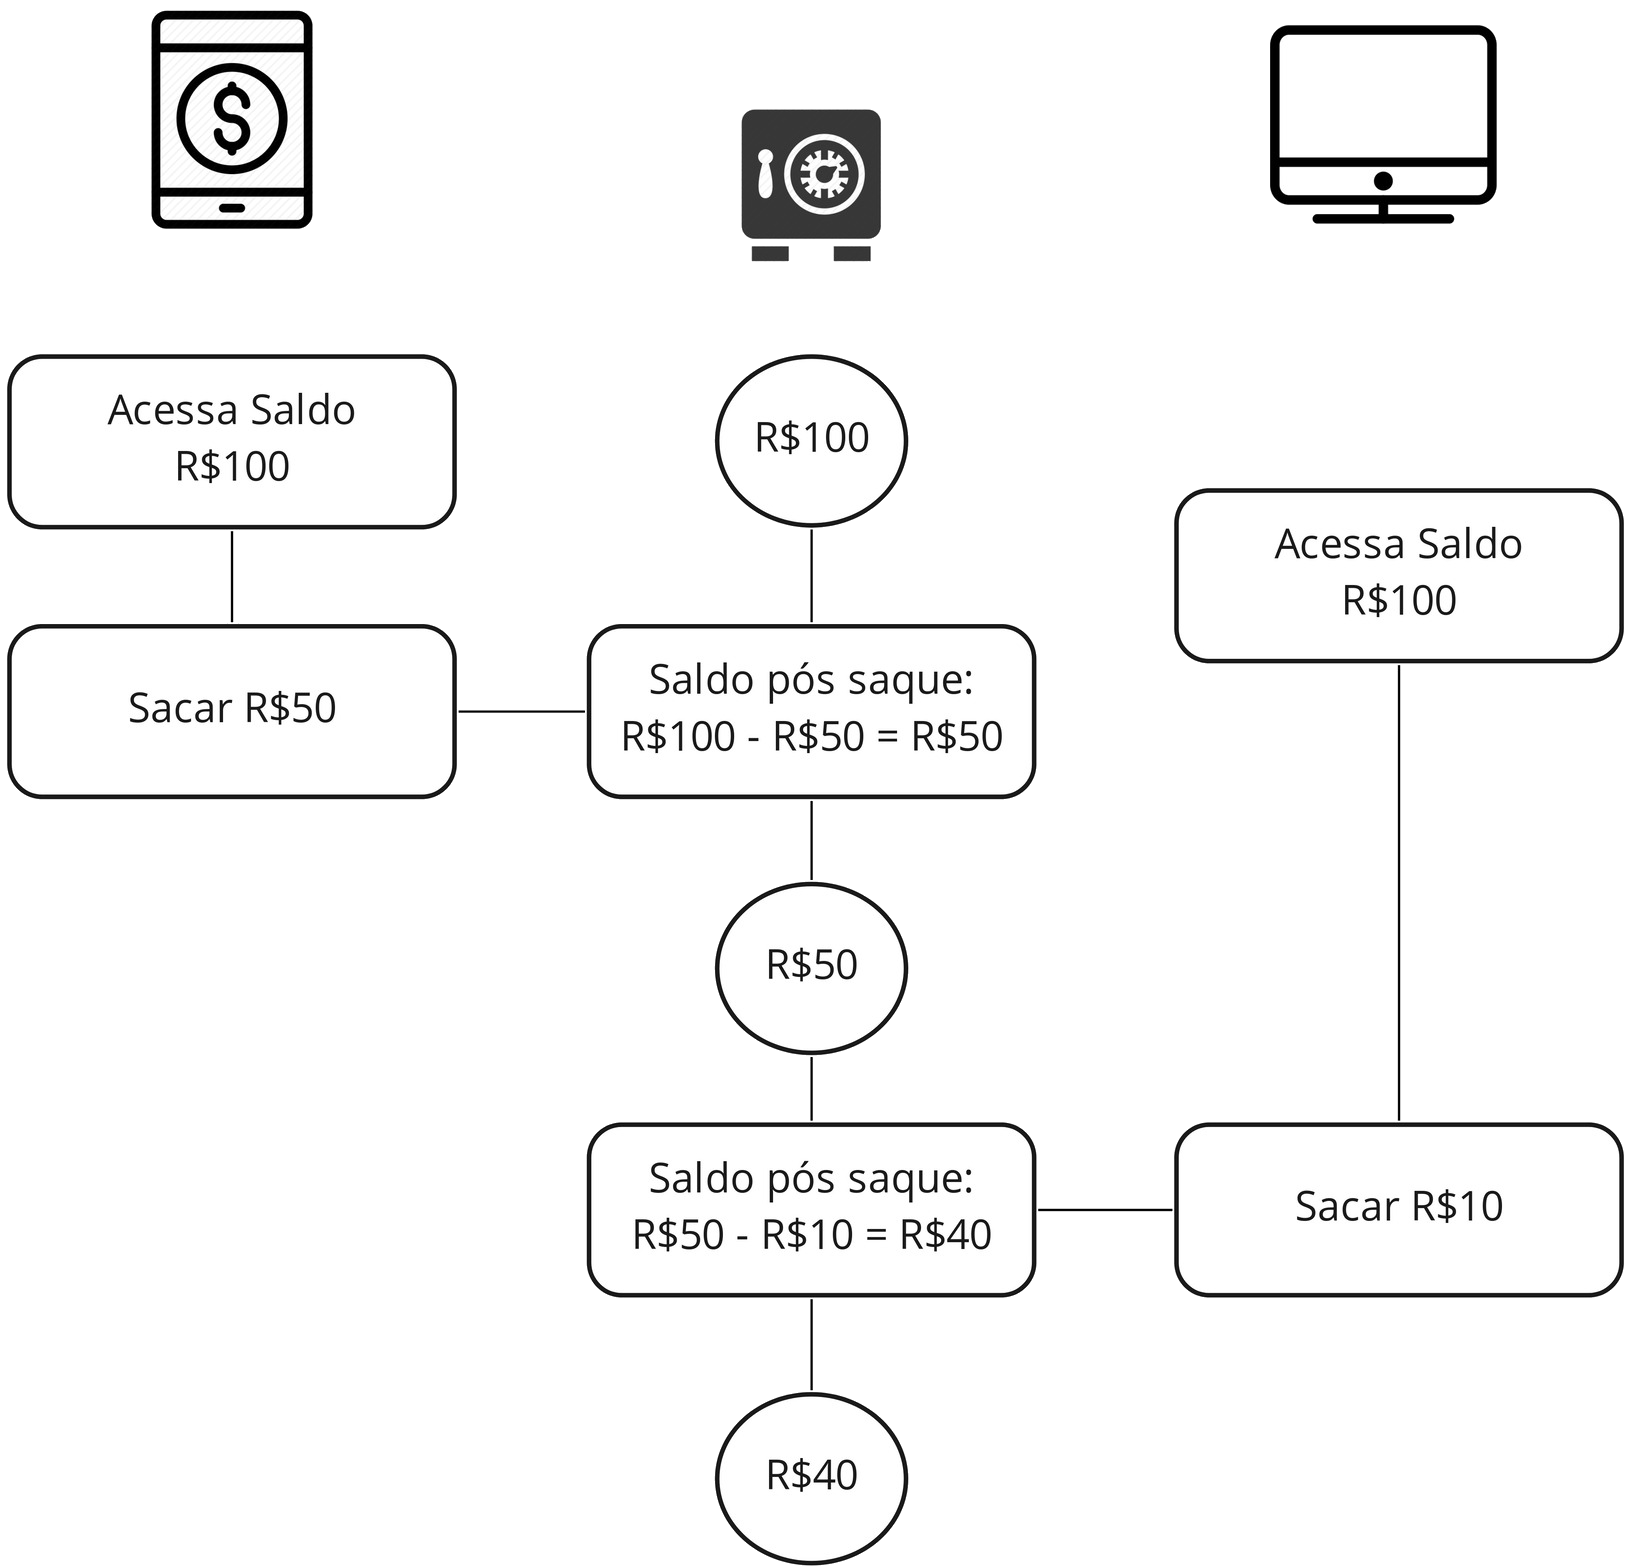
\includegraphics[scale=0.12]{img/bank2.png}
  \end{minipage}
  \hfill
  \begin{minipage}{0.3\textwidth}\centering
    Modelos são sequenciais.\\\medskip
    Ordem das ações pode ser não determinística\\\medskip
  \end{minipage}
\end{frame}

\begin{frame}
  \frametitle{Não determinismo centralizado em um oráculo}
  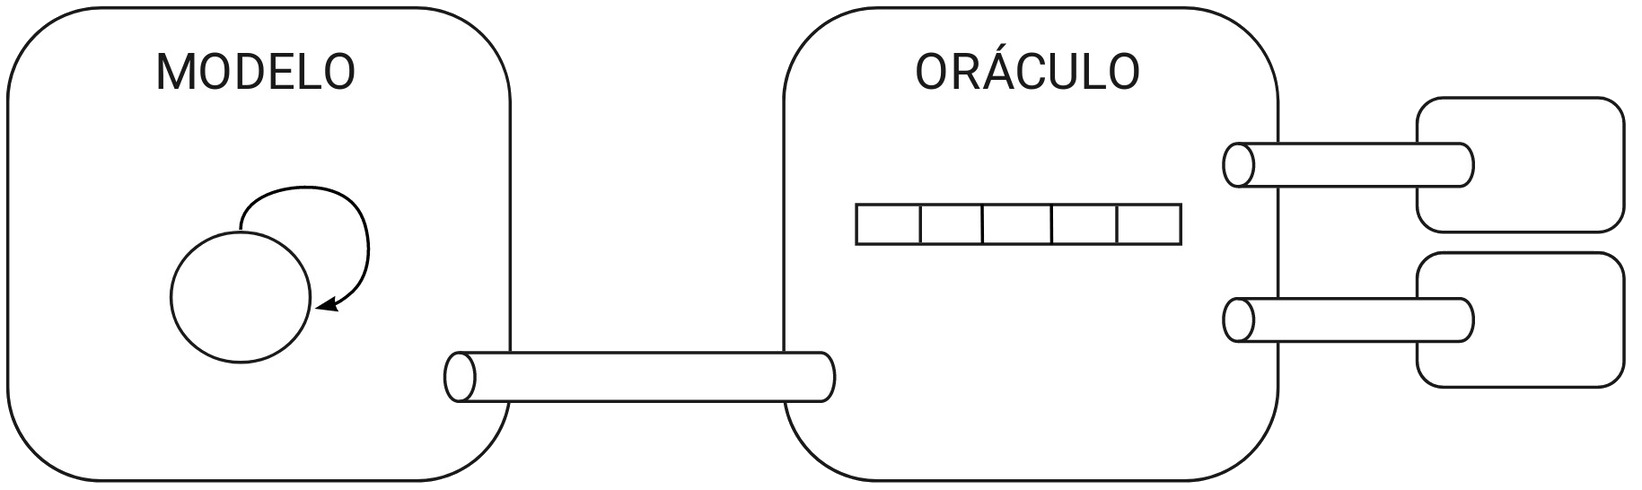
\includegraphics[scale=0.18]{img/diagram.png}\\
  Quando o modelo não é capaz de decidir o próximo estado (como no caso de
  $saldo = 60$), é delegada uma escolha ao oráculo, que centraliza toda a
  influência externa no modelo.
\end{frame}  

\begin{frame}
  \frametitle{Por que Elixir?}

  \begin{enumerate}
    \item Concorrência: gera \textit{bytecode} da máquina virtual do Erlang (BEAM).

    \item Paradigma funcional: se aproxima de definições matemáticas, proporcionando um complexidade menor para as traduções.

    \item Expressividade: código entendível, permitindo alta manutenabilidade.

    \item Transparência de plataforma

    \item Open Source

  \end{enumerate}
\end{frame}

\section{Próximos passos}

\begin{frame}
  \frametitle{Considerações}

  Até aqui:
  \begin{itemize}
    \item Estudo dos construtores de \TLA e entendimento da lógica.
    \item Validação da estrutura inicial do código traduzido.
    \item Início da listagem de mapeamentos.
  \end{itemize}

\end{frame}

\begin{frame}
  \frametitle{Próximos passos}

  A continuidade do trabalho será feita em duas frentes paralelas:
  \begin{itemize}
    \item Busca por mais mapeamentos
    \item Implementação do tradutor (em Haskell)
  \end{itemize}\medskip\pause

  \begin{block}{Exploração}
    \begin{itemize}
      \item Fornecimento de garantias para os mapeamentos
      \item Gerar complementos para melhorar o ambiente de desenvolvimento (e.g. testes unitários)
    \end{itemize}
  \end{block}

\end{frame}

\begin{frame}
  \frametitle{Obrigada!}

  {\Huge Fim :D}\bigskip

  Gabriela Moreira Mafra\\\smallskip
  {\url{gabrielamoreiramafra@gmail.com}}

\end{frame}

\end{document}

